% Generated 2021-02-06 01:28:14 +0530
\subsection{Limits for ProcessSpecification} \label{sec:Limits for ProcessSpecification}


This section provides semantic information for the \block{ProcessSpecification} model.

\begin{figure}[ht]
  \centering
    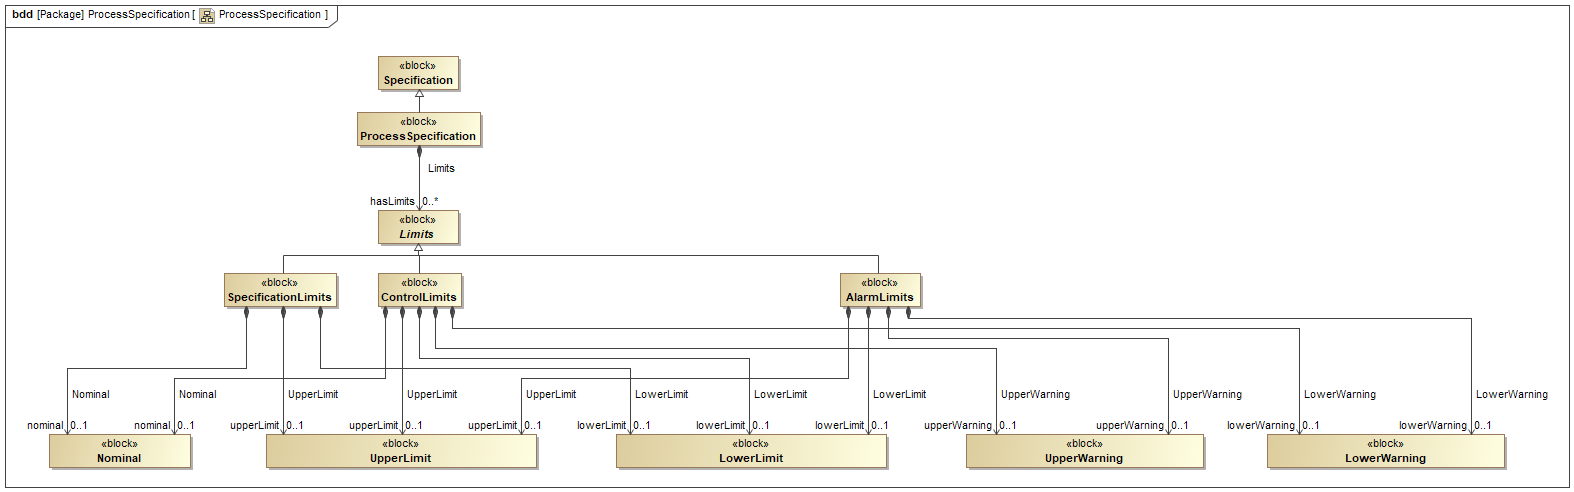
\includegraphics[width=1.0\textwidth]{figures/ProcessSpecification.png}
  \caption{ProcessSpecification Diagram}
  \label{fig:ProcessSpecification Diagram}
\end{figure}

\FloatBarrier


Note: See \fig{ProcessSpecification Schema Diagram} for XML schema.


\subsubsection{Limits}
\label{sec:Limits}



\block{Limits} is an abstract element of \block{ProcessSpecification} that represents a set of conformance boundaries or conditions for a variable.



\subsubsection{AlarmLimits}
\label{sec:AlarmLimits}



A set of limits used to trigger warning or alarm indicators.


\paragraph{Elements of AlarmLimits}\mbox{}
\label{sec:Elements of AlarmLimits}

\tbl{Elements of AlarmLimits} lists the elements of \texttt{AlarmLimits}.

\begin{table}[ht]
\centering 
  \caption{Elements of AlarmLimits}
  \label{table:Elements of AlarmLimits}
\tabulinesep=3pt
\begin{tabu} to 6in {|l|l|} \everyrow{\hline}
\hline
\rowfont\bfseries {Element} & {Multiplicity} \\
\tabucline[1.5pt]{}
\texttt{UpperLimit} & 0..1 \\
\texttt{UpperWarning} & 0..1 \\
\texttt{LowerLimit} & 0..1 \\
\texttt{LowerWarning} & 0..1 \\
\end{tabu}
\end{table}
\FloatBarrier


Descriptions for elements of \block{AlarmLimits}:

\begin{itemize}

\item \block{UpperLimit} \newline The upper conformance boundary for a variable.

Note to Entry: immediate concern or action may be required.


\item \block{UpperWarning} \newline The upper boundary indicating increased concern and supervision may be required.

\item \block{LowerLimit} \newline The lower conformance boundary for a variable.

Note to Entry: immediate concern or action may be required.

\item \block{LowerWarning} \newline The lower boundary indicating increased concern and supervision may be required.
\end{itemize}



\subsubsection{SpecificationLimits}
\label{sec:SpecificationLimits}



A set of limits defining a range of values designating acceptable performance for a variable.


\paragraph{Elements of SpecificationLimits}\mbox{}
\label{sec:Elements of SpecificationLimits}

\tbl{Elements of SpecificationLimits} lists the elements of \texttt{SpecificationLimits}.

\begin{table}[ht]
\centering 
  \caption{Elements of SpecificationLimits}
  \label{table:Elements of SpecificationLimits}
\tabulinesep=3pt
\begin{tabu} to 6in {|l|l|} \everyrow{\hline}
\hline
\rowfont\bfseries {Element} & {Multiplicity} \\
\tabucline[1.5pt]{}
\texttt{UpperLimit} & 0..1 \\
\texttt{Nominal} & 0..1 \\
\texttt{LowerLimit} & 0..1 \\
\end{tabu}
\end{table}
\FloatBarrier


Descriptions for elements of \block{SpecificationLimits}:

\begin{itemize}

\item \block{UpperLimit} \newline The upper conformance boundary for a variable.

Note to Entry: immediate concern or action may be required.


\item \block{Nominal} \newline The numeric target or expected value.

\item \block{LowerLimit} \newline The lower conformance boundary for a variable.

Note to Entry: immediate concern or action may be required.
\end{itemize}



\subsubsection{ControlLimits}
\label{sec:ControlLimits}



A set of limits used to indicate whether a process variable is stable and in control.


\paragraph{Elements of ControlLimits}\mbox{}
\label{sec:Elements of ControlLimits}

\tbl{Elements of ControlLimits} lists the elements of \texttt{ControlLimits}.

\begin{table}[ht]
\centering 
  \caption{Elements of ControlLimits}
  \label{table:Elements of ControlLimits}
\tabulinesep=3pt
\begin{tabu} to 6in {|l|l|} \everyrow{\hline}
\hline
\rowfont\bfseries {Element} & {Multiplicity} \\
\tabucline[1.5pt]{}
\texttt{UpperLimit} & 0..1 \\
\texttt{UpperWarning} & 0..1 \\
\texttt{LowerWarning} & 0..1 \\
\texttt{Nominal} & 0..1 \\
\texttt{LowerLimit} & 0..1 \\
\end{tabu}
\end{table}
\FloatBarrier


Descriptions for elements of \block{ControlLimits}:

\begin{itemize}

\item \block{UpperLimit} \newline The upper conformance boundary for a variable.

Note to Entry: immediate concern or action may be required.


\item \block{UpperWarning} \newline The upper boundary indicating increased concern and supervision may be required.

\item \block{LowerWarning} \newline The lower boundary indicating increased concern and supervision may be required.

\item \block{Nominal} \newline The numeric target or expected value.

\item \block{LowerLimit} \newline The lower conformance boundary for a variable.

Note to Entry: immediate concern or action may be required.
\end{itemize}


